\chapter{Implementation}
\label{chapter:implementation}

This chapter will describe the implementation of the tool.
In particular, we will outline high-level architecture of
the software, discuss internal representation of
LCL problems as well as representation of the query object.
Moreover, we will discuss how batch classification has been
implemented. Finally, in the end of the chapter we will cover
several miscellaneous items such as problem normalization
algorithm, integration of Round Eliminator tool into
our software and some of the properties of the Web interface,
which has also been implemented as part of the thesis project.

\section{General architecture of the tool}

This section will outline general architecture of the tool and
will describe in further detail some of its most important
components. Despite the chapter's name, we are not going
to describe low-level implementation detail in this section,
but instead try to convey technical perspective on the tool
as a whole. We will also discuss and critically analyze some
of the architectural and technological decisions that have been
made during the implementation phase.

On the high level, the software consists of three parts:
front-end application, back-end application and a database.
The database contains arguably the most important component
of this project -- definitions of LCL problems as well as their
known upper and lower bounds. The back-end part contains
the core logic for classifying LCL problems. Besides, it acts
as a middle layer between the database and the front-end part.
That is, it is responsible for receiving data from one of the
components (e.g.\ database), transforming it to the
format understandable by the other part (e.g.\ the front end),
and finally sending it to that part. Finally, the
front-end part's main responsibility is to provide
an understandable and user-friendly user interface
through which one could classify individual LCL problems
as well as query for the whole families of problems
that satisfy specified criteria. Furthermore,
the client-side part of the application is
responsible for displaying the results returned by the
back-end part in a concise and understandable manner.

\begin{figure}[ht]
  \begin{center}
    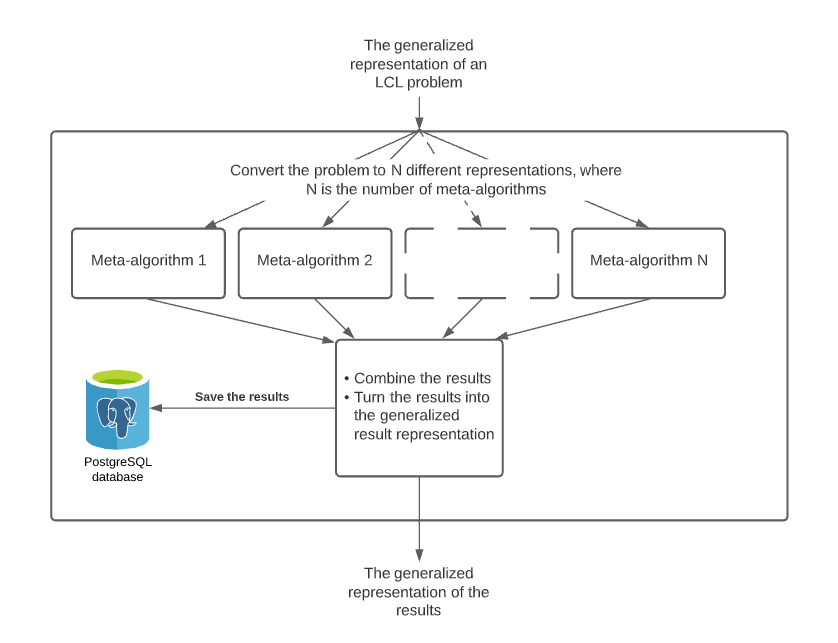
\includegraphics[width=\textwidth]{images/tool-architecture.png}
    \caption{High-level architecture of the implementation}
    \label{fig:implementation-architecture}
  \end{center}
\end{figure}

The database contains only three tables: one for
storing LCL problems together with their upper and
lower bounds, one for keeping track of what families of
problems have been generated and classified via batch
classification mechanisms, and one storing meta-data
of the meta-algorithms used in classifying the LCLs.
The front end is quite simple from technical perspective
too. Some of the details about the client side of the
application will be discussed more in Section~\ref{section:webinterface}.
The back end, however, contains most of the compplexity of
the tool. Therefore, in this section, we will concentrate
mainly on the sever side.

\subsection{Problem}

The core element of the whole application and of the
back-end part in particular is the Problem class.
For representing an LCL problem, we have decided
to use notation similar to that of Round
Eliminator. Our representaion however also
allows for graph types other than trees -- namely cycles.
Besides, it allows the underlying graph of a problem
to be rooted (or directed in the case of cycles).
Finally, it allows representing problems where
leaves' and root's output labels are also constrained.
The representaion similar to that of a Round
Eliminator has been chosen because of its generality.
In particular, as we have shown in Theorem~\ref{theorem:re_formalism_is_general},
any LCL problem
on $(\beta, \delta)$-biregular unrooted trees -- provided
that nodes of degrees other than $\beta$ and $\delta$ are unconstrained
and nodes near leaves are unconstrained -- can be represented
using the formalism used in the Round Eliminator.

Since we are only concerned with problems on regular trees and cycles
this representation works well for us. For the cases of cycles,
the only restriction is that degree of both passive and
active configurations has to be two. Also, the case
of directed (rooted) cycles (trees) can be handled
using the \emph{colon notation} that has been already
previously used in a recent paper on automating
the classification of LCLs in rooted trees~\cite{Balliu2021}.
Furthermore, the cases when \emph{irregular} nodes, i.e.\ leaf
nodes or root node, are restricted can also
be handled by specifying those restrictions
(separately for leaf nodes and a root node)
as separate properties of the Problem object.
Thus, our representation of LCL problems is general
enough to cover all the LCL problems that are
included in the scope of the project.

Having explained this, we can finally list all the
properties that are encapsulated into the
Problem object. The object contains the already
mentioned active configuration, passive configurations,
leaf constraints (which can be an empty set), root constraints
(which can be an empty set too), as well as special flag variables
indicating whether all active or all passive configurations
are allowed for active and passive nodes respectively.
If one of the two flag variables are set to true,
it overrides whatever is contained in the variables
holding the actual active and passive configs.
Besides, each problem object contains information
on the type of the underlhing graph: path, cycle or
tree. Notice that although any path is always a tree,
we chose to differentiate between those two
for convinience. It is worth mentioning that
a path graph type will be chosen as internal
representation whenever both active and
passive configurations are of degree two and
the user-selected graph type is not cycle.
In particular, if a user specifies tree as a graph
type and provides configurations of degree two,
tree will still be chosen as a graph type of the problem
internally. Finally, after parsing the configs
that are always provided in a string format,
the tool automatically decides whether the given problem's
underlyhing graph is rooted/directed or not.

It is also worth noting that as a first step of
creating a Problem object, the specified parameters,
including nodes' configurations and constraints
are checked for validity. Thus, if, for example,
a problem is misspecified so that some of the
configurations are ``directed'' while others are not,
an exception is thrown containing a message with
a human-readable explanation for why the
specification was invalid. After the validity
of the specification is checked, a problem is
normalized by executing the normalization algorithm
described below in Section~\ref{section:problem-normalization}.

\subsection{Classification}

Another central component of the back end is
the function responsible for classification of LCL problems.
On the high level, the function takes as input an LCL problem and
runs underlying meta-algorithms, some of which might be
able to provide some useful information about the complexity of the
problem. After that, the function combines the results
returned by all the meta-algorithms. Based on teh results returned,
the function determines the tightest known lower and upper bounds of
the LCL problem both in the deterministic and randomised LOCAL
models. Finally, a Response object is constructed based on the bounds
and is returned as the functions result. In the best case, tight
complexity bounds are found for both deterministic and randomized
settings. In the worst case, trivial bounds are returned:
``unsolvable'' for upper bounds and $\Omega(1)$ for lower bounds.

Each of the underlying meta-algorithms or datasets is wrapped
in a function -- we will refer to it as ``subclassify'' from now on -- such
that it provides unified interface for the main
``classify'' function. In particular, subclassify takes
as input an instance of the Problem class and
returns an instance of Response class. A Response object
simply encapsulates upper and lower bounds for both
deterministic and randomized settings. There is
exactly one subclassify function for each meta-algorithm
or dataset that we use. Inside each subclassify function,
we first check if the provided problem can be classified
at all by the underlyinng meta-algorithm. Often, we can
exit early already at this stage if, for examle, the meta-algorithm
in question deals only with rooted trees and the provided input is a 
problem on unrooted trees (or e.g.\ a problem on cycles). Then,
if we haven't exited the function yet,
we transform an instance of the Problem class to a problem
representation used by the meta-algorithm that the given
subclassify wraps around. The meta-algorithm is then executed,
the retured result is transformed into an instance of the
Response class and the Response object is returned as
a result of the subclassify function.

\subsection{Query}

The query class encapsulates some of the properties
based on which the database is queried for problems.
Only problems that satisfy the provided Query object will be
returned. The properties encapsulated by a Query object are
more or less directly mapped to an SQL query's WHERE clause.
The Query class groups those properties in three parent items:

\begin{itemize}
  \item problem properties,
  \item complexity bounds,
  \item include/exclude configuration.
\end{itemize}

\emph{Problem properties} define a class of problems that are to be
returned from the database. It includes the following fields:

\begin{itemize}
  \item active degree,
  \item passive degree,
  \item alphabet size (upper bound on it to be precise),
  \item Whether active/passive configurations are necessarily monochromatic,
  \item Whether underlyig graph directed/rooted or not,
  \item Type of the underlying graph. Which is always one of the following three
  options: tree, cycle, path.
\end{itemize}

\emph{Complexity bounds} limit the returned problems further by
restricting their complexities. The \emph{complexity bounds} object
contains the following items:

\begin{itemize}
  \item upper bound in randomized LOCAL setting (referred to as RUB),
  \item lower bound in randomized LOCAL setting (referred to as RLB),
  \item upper bound in deterministic LOCAL setting (referred to as DUB),
  \item lower bound in deterministic LOCAL setting (referred to as DLB).
\end{itemize}

The restriction of the fetched problems is done according to the
following logic: only those problems are returned (not filtered out)
whose known randomized upper bound is at most as high as RUB, whose
known randomized lower bound is at least as high as RLB, whose
known deterministic upper bound is at most as high as DUB and whose
known deterministic lower bounds is at least as high as DLB. Notice that
for a problem not to be filtered out, all the four criteria must be
satisfied.

Finally, \emph{include/exclude configuration} has the following
items encapsulated in it:

\begin{itemize}
  \item Whether only ``smallest'' problem has to be returned (in terms of the number of configurations).
  \item Whether only ``largest'' problem has to be returned (in terms of the number of configurations).
  \item Whether only those problems must be returned whose randomised upper
  and lower bounds do not match.
  \item Whether only those problems must be returned whose deterministic upper
  and lower bounds do not match.
  \item Whether only those problems must be returned whose randomised both
  upper and lower bounds are trivial (i.e.\ unsolvable and $\Omega(1)$
  respectively).
  \item Whether only those problems must be returned whose deterministic both
  upper and lower bounds are trivial (i.e.\ unsolvable and $\Omega(1)$
  respectively).
  \item List of configurations $L$ such that if a problem's configurations contain at least one configuration from $L$, the problem is excluded. Note
  the item has not effect if left empty.
  \item List of configurations $L$ such that if a problem's configurations contain all of the configuration from $L$, the problem is excluded. Note
  the item has not effect if left empty.
  \item List of configurations $L$ such that if a problem's configurations contain at least one configuration from $L$, the problem is included.
  Otherwise a problem is excluded.
  Note
  the item has not effect if left empty.
  \item List of configurations $L$ such that if a problem's configurations contain all of the configuration from $L$, the problem is included.
  Otherwise a problem is excluded.
  Note
  the item has not effect if left empty.
\end{itemize}

\section{Problem normalization}
\label{section:problem-normalization}

This section describes the above mentioned problem normalization
algorithm. The algorithm is used for determining which problems
are equivalent to each other. This, in turn, allows us
to reduce the amount of needed storage. Besides, this prevents
situtaions when a tool needs to run classification for a problem $A$
from the very beginning while an isomorphic problem $B$ has already been classified
by the tool previously and saved in the database. Thus, the normalization
algorithm also allows us to reduce the usage of computational resources.

The algorithm is based on the problem normalization algorithm
from Round Eliminator~\cite{Olivetti2020}. While the original
algorithm is written in Rust programming language, I
reimplemented it in Python and changed some of its
implementation details to better suit our purpose.
However, the general idea of the algorithm stays the same.

First, we determine how many labels are used in the description of the
problem $P$ i.e.\ its alphabet size. Then, we map each letter in the description
to a letter from A to Z. For example, if numbers were used for describing
the problem, the numbers will be mapped to capital letters of
English alphabet. It is important to point out already now that
one limitation of the current implementation is the fact that
a problem with more than 26 labels cannot be correctly normalized.
Once we obtain the list of letters used, we calculate all
permutations of the list. For each permutation, we execute the following
subroutine:

\begin{itemize}
  \item Based on the given permutation, create a mapping from each
  element of the problem's alphabet to each symbol in the permutation.
  That is, we map the $i$'th letter of the $P$ alphabet to the $i$'th symbol
  in the permutation for all $i$ from 1 to the size of $P$'s alphabet.
  \item Based on the obtained mapping, do the following with the problem's
  active configurations, passive configurations, leaf constraints and
  root constraints one at a time.
  
  \begin{itemize}
    \item For each line of the configurations/restrictions, rename symbols
    according to the mapping constructed above.
    \item If the problem $P$ is specified on unrooted/undirected graph,
    change position of all symbols on each line of the configurations/restrictions according to symbols alphabetical order.
    If the underlying graph of $P$ is directed/rooted, keep the currently first
    symbol as first, but change positions of all the rest symbols (again separately for each line)
    according to symbols alphabetical order.
    \item If at this point, some configuration lines are
    duplicated, remove all the duplicates so that each configuration
    line is unique.
    \item Sort the unique configuration lines in alphabetical order
    treating the lines as strings.
  \end{itemize}

  \item Return the newly constructed active configurations,
  passive configurations, leaf constraints and root constraints as
  a tuple of four elements.
\end{itemize}

Each execution of the subroutine described above yields a tuple
of size four. Thus, after executing the subroutine on each permutation of
labels, we eventually obtain a list of tuples of size four.
Then we sort the list, and take its first element. The four
tuple's elements are then assigned to the $P$'s
active configurations, passive configurations, leaf
constraints and root constraints respectively.

% \begin{algorithm}
% \DontPrintSemicolon
% \caption{\label{alg:normalize}normalize($P$)}
% \KwIn{problem $P$}
% \KwOut{problem $P$ with its constraints and configurations normalized}

% $lc \gets$ number of labels in $P$ \;
% $ls \gets$ first $lc$ capital letters of English alphabet \;
% $perms \gets$ a list of all permutations of $ls$  \;
% $all_normalized \gets$ empty array \;
% \For{every $perm$ in $perms$} {
%     add $normalizeForPermutation()$ $all_normalized \;
% }

% this is just an example 


% \Repeat{$R_{i} = R_{i-1}$}{
%   $i \gets i + 1$\;
%   $R_{i} \gets R_{i-1}$\;
  
  
% \uIf{$(\Sigma_\Pi,a \neq \epsilon) \in R_i$ and $\Pi$ is non-empty}{
%   \Return $\Sigma$
%   }
% \Else{
%   \Return $\epsilon$
% }
% \end{algorithm}


\section{Batch classification and reclassification}

This section describes how batch classification and
batch reclassification mechanisms have been implemented.
Batch classification is important since we want our database
to be prepopulated with significant number of classified
problems already before the first users start using it.
In particular, we would need to classify huge but finite
families of problems consisting of tens and hundreds of
thousands of LCL problems. Moreover, once a family of
problems is selected, the problems of the famnily need to
be generated and turned into instances of Problem class before
we can actually classify them. Batch reclassify functionality,
on the other hand, is needed for cases when, for one reason
or another, we would want to reclassify a certain
family of LCL problems that is already stored in our
database. For example, if we integrate a new meta-algorithm
to our solution in the future, we would need to reclassify
all problem families that are compatible with the newly-integrated
meta-algorithm. Or purhaps, a programming mistake has been
made when integrating one of the meta-algorithms, and therefore,
the problems need to be reclassified again.

One option for implementing batch reclassification
mechanisms would be to simply delete all of the problems
of the class in question from the database and execute
the batch classificatoin logic from the beginning
including its first step of generating the problems
of the problem class. However, this is suboptimal,
since generation of problems of a certain family
usually takes significantly longer times than
the subsequent classification step. For this reason,
we decided to have separate functionality for
batch reclassification.

The batch classification process starts with creating
an object that specifies a family of problems to be
generated, classified and stored in the database.
The specification includes properties like
active and passive degrees, label count, type of the
underlying graph, etc. The problems of the given
family are then generated via the following algorithm:

\begin{enumerate}
  \item Based on the specified label count, get a list of
  all symbols i.e.\ alphabet of the problem family
  \item Based on the alphabet and the specified active/passive
  degrees, generate lists of all the possible
  active and passive one-line configurations
  \item Get a list of all possible combinations
  of active one-line configurations and a list of all possible
  combinations of passive one-line configurations. The combinations
  can be of any size. This can be accomplished via
  the ``powerset'' function. Now we have lists of
  all possible active and passive configurations.
  \item Remove configurations that are empty.
  \item Generatate all possible tuples of size two
  where the first element is an active configuration and
  the second is a passive configuration. This corresponds
  to cartesian product between the previousy generated
  lists of all active and passive configurations.
  \item Remove tuples that have exact duplicates in the
  gnerated list of tuples, so that all tuples are unique.
  \item Turn each tuple into a Problem object using
  elements of the tuple as active and passive configurations.
  \item Normalize all the problems
  \item Now that all the problems are in a normalized 
  representation, it is easy to detect whether any two
  problems are isomorphic to each other. Remove such
  problems from the list so that the list contains only
  unique non-isomorphic problems.
  \item Return the list of newly-generated problems.
\end{enumerate}

Once the problems are generated, we store them to the database,
even though they are not classified yet. This is done mainly
because the database will automatically associate a unique
identifier with each of the problems.

After that, the problems are classified. Notice that
some of the meta-algorithms provide a way to classify
lists of problems at the same time, which is often
significantly faster than classifying one problem at a time.
This is due to the fact that some meta-algorithms
(e.g.\ TLP classifier and BRT classifier) are in fact
huge datasets of preclassified problems. When
classifying each problem individually, such
meta-algorithms would need to read out the whole
dataset from the disk, find one specific problem,
and return the result. On the other hand, when
classifying multiple problems at the same time,
numerous optimizations can be applied e.g.\ reading the 
dataset from the disk just once and search for all
requested problems at the same time. For this reason,
when batch classifying families of problems we first
call such batch classiicatio methods of meta-algorithm
if such methods exist. Once this is done, a modification
of the previously-described classify function is called
for each individual Problem object. The difference is
that if a meta-algorithm $A$'s batch classify method has been
already called, its ``subclassify'' function is not called
anymore during the individual-problem classification which
can significantly speedup the whole batch classification
functionality. Finally, when all problems have been classified,
the database is updated with the classification results.

The batch reclassification functionality resembles
what has been described above with the excpetion that,
once a family of problems has been specified, it is
not generated but is instead queries from the database.
After that, the fetched problems undergo the same
batch classification process. Finally, the database is
updated with the received classifications.

\section{Integration of Round Eliminator}

This section describes how the Round Eliminator
tool~\cite{Olivetti2020} has been integrated in our solution.
Prior to integration we had had considered several options:

\begin{itemize}
  \item Using an API of a server that runs the back end of the Round Eliminator tool
  \item Calling REtor as a command line tool from our Python
  application and then parsing the output, which is returned
  in a text format as part of stdout~\cite{stdio}
  \item Compiling REtor's source code to a ``Shared Object'' file (.so extension)
  using CPython ~\cite{CPython} bindings and then importing the compiled
  functions to our Python application as CPython dependency.
\end{itemize}

At the moment of writing the thesis, the Round Eliminator tool
is deployed using WASM~\cite{WASM}. This virtually means that
there is no back-end part running on a server, but instead
all of the logic is executed on the client side of the application.
Redeploying the tool with a standalone server and a separate client
part did not seem like a feasible alternative since this would
require a nontrivial amount of work from the tool's maintainers.
Thus, the first option was not feasible.

On the other hand, the second option was feasible. Indeed,
this method of using REtor had already been used in the
implementation of TLP Classifier~\cite{Rocher2020clas}. However,
this approach has several crucial disadvantages.
Firstly, the overhead of calling a command line command
from a Python program is significant compared to just calling
a Python function. Secondly, the output of Round Eliminator
would have to be parsed from the plain textual format, which
would have added an additional complexity of the software.
Finally, the approach complicates distribution and deployment of
the software. Indeed, one would have to install the specific
version of Rust programming language as well as download and
build form source codes the specific version of REtor required.

Instead, we have decided to go with the latter option. This
alternative does not have any of the disadvantages listed
in the previous paragraph while being just as feasible and
easy to implement. Compiled in this manner, the whole of
Round Eliminator logic is contained in a single .so file
that can be easily deployed to e.g.\ a production server.
Besides, the speed improvement is significant: we were
able to execute up to three rounds of round eliminator
in under 100 milliseconds. Finally, the functions
exposed via the .so file, return python-native
data structures so that no additional parsing is required on our side.
This, in turn has been achieved by adding CPythin bindings
to the REtor source code. The bindings wrap the relevant functions
written in Rust, thus enabling us to pass Python data structures
as parameters and recieve the return values as python-interpretable values.
The bindings were implemented using the rust-cpython library~\cite{RustCPython}.


\section{Web interface}
\label{section:webinterface}

This section will briefly discuss some implementation details of
the client side of the application. First, we start explaining why
the web interface has been implmented in the first place and why it
is important. Then, we describe some of the technologies that were
chosen as part of the implementation. Finally, we describe the
reasoning behind and advantages of the forms' state being stored
as a query part of the URL.

The reason why we decided to spend additional time and implement
the web interface can be best unnderstood when considering
another tool that has recently been rising in popularity among
the distributed algorithms community -- Round Eliminator~\cite{Olivetti2020}. The tool has proved to be a very useful utility
when doing research connected to LCL problems on biregular trees.
However, if it wasn't for the web interface that Olivetti has
implemented, it is most likely that the popularity and
frequency of use of the tool would have been nowhere near the current
levels. Indeed, almost all users of the tool use it via the web
client. Otherwise, a user would need to install Rust programming
language~\cite{Rust}, build the tool locally using the tool
called ``Cargo''~\cite{Cargo} and then run it using the command-line.
It is clear that the number of people willing to do that would be
significantly smaller than number of people who ended up using
an easy-to-use web interface that requires no installation or 
configuration.

By analogy, we can assume with high confidence that significantly more
user would be willing to use our tool vie the web interface rather
than downloading the soource of the tool locally and installing
a specific version of Python programming language~\cite{CPython}.
Moreover, the richness of the web user interface allows us to convey complicated
ideas related distributed computing in way that is easier to understand, at least for knowledgable audience. Thus, it is has been
decided to spend some time resources -- even though they were 
quite limited -- on implementing a web user interface that is
relatively easy to use and understand compared to its
command line -based analog.

The web interface consists of two forms. One form for classifying
individual problems, and another one for issueing queries
about groups of problems against the database. When using the
first form, our application will first check if the requested
problem can be found in a database. If not, it will proceed to
running the classifiers (which corresponds with the ``classify'' function described above) and will eventially return the newly
classified result. If the classification result is not trivial (which means that lower bounds are constant and upper bounds are unsolvable),
it will also be stored in the database. The second ``query'' form, once
submitted will be transformed into the previously described
``Query'' object. The query will then be executed against the database,
the results will be returned to the client side and rendered
in a user-friendly format.

As a programming language for our front-end application, we decided
to use TypeScript~\cite{TypeScript}. TypeScript is a general purpose
programming language developed and maintained by Microsoft. It is closely related to JavaScript programming language, which has become de facto standard programming language for the Web.
As a framework for our client application, we have decided to use
Svelte~\cite{Svelte}. Svelte is an open-source front-end framework
written in TypeScript. Among other things, it allows a simplified
approach for application state management, and reduces initial
page load times compared to other front-end frameworks~\cite{SvelteVsReactBundleSize}.

For the styling of the front end, we used a minimalist CSS framework
called ``Milligram''~\cite{Milligram}. It provides a good starting point
when it comes to styling a modern web application. Besides, the total
size of the framework is just 2 kilobytes when zipped~\cite{Milligram}.
This, simplicity to use, and our previous positive experience with
the framework were the decisive factors that influenced our final
choice.

As a final interesting piece of technology used, we describe properties
and our reason for choosing to use svelte-virtual-list~\cite{svelte-virtual-list}.
The library allows rendering only part of the content instead of rendering
the whole of the content on a web page. In our case, this is
particularly useful as it allows us to
show tens of thousands of LCL problems (returned as part of the described above querying functionality) in a virtual list.
The virtual list, implemented via the above mentioned svelte-virtual-list library, renders only a small number (about 3--4)
LCL problems at the same time. At the same time, it allows user to
scroll through the list of problems with no noticable delay.
If not for the library, our client application would have to render
tens of thousands of LCL problems all at once. This would result in
the user interface freezing for a prologned period (up to several minutes).

Finally, we will explain the reasoning behind and benefits for
storing the state of the two forms as part of the URL's query
component. When searching for interesting query results, or even
just classifying different individual LCL problems, it is often
required to demonstrate the results to somebody else. To allow for such
a sharing, we decided to encode the state of both forms in the URL.
Thus, once e.g.\ the results of a query are obtained, it is possible
to copy the link and simply send it to, for example, a colleague.
When opening the link, both forms will be prefilled with
exactly the same values as those of the sender. This will make sure
that in most cases the sender and the reciever of the link will end
up with the same results displayed. Besides, if a particularly
interesting query has been discovered, it is possible to
simply copy and store the link. Opening the link in the future,
will prefill the forms with the same parameters and display
the same relevant results.

% \section{Deployment details}

% This section will outline some of the details related
% to how the application has been deployed. We will
% describe our high-level setup without listing all the
% details and configurations of each of the services used.

% We host our application on an infrastructure provided by
% CSC - IT Center for Science, Finland~\cite{FIXME}.
% The center provides an OpenStack solution, which is
% an open standard cloud computing software that provides
% infrastructure-as-a-service service. Our software
% is deployed to a virtual instance that was created
% via the OpenStack solution. The database is
% stored on a ``volume'', which unlike virtual instances,
% provide long-term persistent storage.

% FOr 
